\documentclass[a4paper,12pt]{article} % тип документа
% назначить цвета при подключении hyperref
\usepackage[unicode, colorlinks, urlcolor=blue, linkcolor=blue, pagecolor=blue, citecolor=blue]{hyperref} %синие ссылки
%\usepackage[unicode, colorlinks, urlcolor=black, linkcolor=black, pagecolor=black, citecolor=black]{hyperref} % для печати (отключить верхний!)
%\mathtoolsset{showonlyrefs=true} % Показывать номера только у тех формул, на которые есть \eqref{} в~тексте.
%кириллица в формулах
\usepackage[warn]{mathtext}
\usepackage{amsmath}
% report, book

%%% Работа с русским языком % для pdfLatex
\usepackage{cmap}					% поиск в~PDF
\usepackage{mathtext} 				% русские буквы в~фомулах
\usepackage[T2A]{fontenc}			% кодировка
\usepackage[utf8]{inputenc}			% кодировка исходного текста
\usepackage[english,russian]{babel}	% локализация и переносы
\usepackage{indentfirst} 			% отступ 1 абзаца
\usepackage{comment}

%%% Работа с русским языком % для XeLatex
%\usepackage[english,russian]{babel}   %% загружает пакет многоязыковой вёрстки
%\usepackage{fontspec}      %% подготавливает загрузку шрифтов Open Type, True Type и др.
%\defaultfontfeatures{Ligatures={TeX},Renderer=Basic}  %% свойства шрифтов по умолчанию
%\setmainfont[Ligatures={TeX,Historic}]{Times New Roman} %% задаёт основной шрифт документа
%\setsansfont{Comic Sans MS}                    %% задаёт шрифт без засечек
%\setmonofont{Courier New}
%\usepackage{indentfirst}
%\frenchspacing

%%% Дополнительная работа с математикой
\usepackage{amsfonts,amssymb,amsthm,mathtools}
\usepackage{amsmath}
\usepackage{icomma} % "Умная" запятая: $0,2$~--- число, $0, 2$~--- перечисление
\usepackage{upgreek}

%%% Страница
\usepackage{extsizes} % Возможность сделать 14-й шрифт

%% Шрифты
\usepackage{euscript}	 % Шрифт Евклид
\usepackage{mathrsfs} % Красивый матшрифт

%% Свои команды
\DeclareMathOperator{\sgn}{\mathop{sgn}} % создание новой конанды \sgn (типо как \sin)
\usepackage{csquotes} % ещё одна штука для цитат
\newcommand{\pd}[2]{\ensuremath{\cfrac{\partial #1}{\partial #2}}} % частная производная
\newcommand{\abs}[1]{\ensuremath{\left|#1\right|}} % модуль
\renewcommand{\phi}{\ensuremath{\varphi}} % греческая фи
\newcommand{\pogk}[1]{\!\left(\cfrac{\sigma_{#1}}{#1}\right)^{\!\!\!2}\!} % для выражений для погрешности

% Ссылки
\usepackage{multirow}
\usepackage[table,xcdraw]{xcolor}
\usepackage{color} % подключить пакет color
% выбрать цвета
\definecolor{BlueGreen}{RGB}{49,152,255}
\definecolor{Violet}{RGB}{120,80,120}



%% Перенос знаков в~формулах (по Львовскому)
\newcommand*{\hm}[1]{#1\nobreak\discretionary{}
	{\hbox{$\mathsurround=0pt #1$}}{}}

%%% Работа с картинками
\usepackage{graphicx}  % Для вставки рисунков
\graphicspath{{images/}{images2/}}  % папки с картинками
\setlength\fboxsep{3pt} % Отступ рамки \fbox{} от рисунка
\setlength\fboxrule{1pt} % Толщина линий рамки \fbox{}
\usepackage{wrapfig} % Обтекание рисунков и таблиц текстом
\usepackage{multicol}

%%% Работа с таблицами
\usepackage{array,tabularx,tabulary,booktabs} % Дополнительная работа с таблицами
\usepackage{longtable}  % Длинные таблицы
\usepackage{multirow} % Слияние строк в~таблице
\usepackage{caption}
\captionsetup{labelsep=period, labelfont=bf}

%%% Оформление
\usepackage{indentfirst} % Красная строка
\setlength{\parskip}{0.3cm} % отступы между абзацами

%%% Теоремы
\theoremstyle{plain} % Это стиль по умолчанию, его можно не переопределять.
\newtheorem{theorem}{Теорема}[section]
\newtheorem{proposition}[theorem]{Утверждение}

\theoremstyle{definition} % "Определение"
\newtheorem{definition}{Определение}[section]
\newtheorem{corollary}{Следствие}[theorem]
\newtheorem{problem}{Задача}[section]

\theoremstyle{remark} % "Примечание"
\newtheorem*{nonum}{Решение}
\newtheorem{zamech}{Замечание}[theorem]

%%% Правильные мат. символы для русского языка
\renewcommand{\epsilon}{\ensuremath{\varepsilon}}
\renewcommand{\phi}{\ensuremath{\varphi}}
\renewcommand{\kappa}{\ensuremath{\varkappa}}
\renewcommand{\le}{\ensuremath{\leqslant}}
\renewcommand{\leq}{\ensuremath{\leqslant}}
\renewcommand{\ge}{\ensuremath{\geqslant}}
\renewcommand{\geq}{\ensuremath{\geqslant}}
\renewcommand{\emptyset}{\varnothing}
\newcommand{\specialcell}[2][c]{%
	\begin{tabular}[#1]{@{}c@{}}#2\end{tabular}}
\usepackage{graphicx}%Вставка картинок правильная
\usepackage{float}%"Плавающие" картинки
\usepackage{wrapfig}%Обтекание фигур (таблиц, картинок и прочего)

%%% Название разделов
\usepackage{titlesec}


% новая команда \RNumb для вывода римских цифр
\newcommand{\RNumb}[1]{\uppercase\expandafter{\romannumeral #1\relax}}

% Цвета для гиперссылок
\definecolor{linkcolor}{HTML}{799B03} % цвет ссылок
\definecolor{urlcolor}{HTML}{799B03} % цвет гиперссылок
 
\hypersetup{pdfstartview=FitH,  linkcolor=linkcolor,urlcolor=urlcolor, colorlinks=true}

\usepackage[left=1.27cm,right=1.27cm,top=1.7cm,bottom=2cm]{geometry}

% нестандартные подписи 
\addto\captionsrussian{\def\chaptername{Глава}} 
\addto\captionsrussian{\def\contentsname{Содержание}} 
\addto\captionsrussian{\def\listfigurename{Список рисунков}} 
\addto\captionsrussian{\def\listtablename{Список таблиц}} 
\addto\captionsrussian{\def\abstractname{Аннотация}} 
\addto\captionsrussian{\def\refname{Список использованных источников}} 
\addto\captionsrussian{\def\indexname{Предметный указатель}} 
\addto\captionsrussian{\def\figurename{Рисунок}} 
\addto\captionsrussian{\def\tablename{Таблица}} 
\addto\captionsrussian{\def\partname{Часть}} 
\addto\captionsrussian{\def\appendixname{Приложение}}

%%% Органическая химия
\usepackage{chemfig}
\usepackage{xymtex}
%\usepackage{ochem}

%%% Фичи
\usepackage{cancel} % Диагональное и Х-зачёркивание
\usepackage{ulem} % Различные типы подчёркиваний
%\usepackage{mathrsfs} % Каллиграфия \mathscr{}

\usepackage{tikz}
\usepackage{boondox-cal} %Каллиграфия \mathcal{x}
%\usepackage{mathptmx}
\usepackage{enumitem}

\usepackage{fancyhdr}
\pagestyle{fancy}
\fancyhf{}
\lhead{4.3.2А Дифракция света на звуковой волне в жидкости}
\rhead{Нестеренко В.В.}
\cfoot{-\thepage -}

\begin{document} % начало документа
 
% НАЧАЛО ТИТУЛЬНОГО ЛИСТА
\begin{center}
\thispagestyle{empty} % выключаем отображение номера для этой страницы
\hfill \break
{МИНИСТЕРСТВО НАУКИ И ВЫСШЕГО ОБРАЗОВАНИЯ РОССИИ}\\
\footnotesize{ФЕДЕРАЛЬНОЕ ГОСУДАРСТВЕННОЕ АВТОНОМНОЕ ОБРАЗОВАТЕЛЬНОЕ}\\ 
\footnotesize{УЧРЕЖДЕНИЕ ВЫСШЕГО ОБРАЗОВАНИЯ}\\
\small{\textbf{«МОСКОВСКИЙ ФИЗИКО-ТЕХНИЧЕСКИЙ ИНСТИТУТ (НАЦИОНАЛЬНЫЙ ИССЛЕДОВАТЕЛЬСКИЙ УНИВЕРСИТЕТ)»}}\\
\hfill \break
\normalsize{ФРКТ}\\
\hfill \break
\hfill \break
\hfill \break
\hfill \break
\hfill\break
\hfill\break
\line(1,0){5030}\\[1mm]
\Large\textbf{{Лабораторная работа № 4.3.2А}}\\
\Large{Дифракция света на звуковой волне в жидкости}\\
\line(1,0){5030}\\[1mm]
\hfill \break

\hfill \break
\end{center}
 
\begin{flushright}
{Выполнил:}

{{\Large Нестеренко Владислав Витальевич}}\\

{группа Б01-009}
\end{flushright}

\begin{figure}[H]
\centering
\includegraphics[scale=0.3]{logo}
\end{figure}
\begin{center} Долгопрудный,  \today \end{center}
\thispagestyle{empty} % выключаем отображение номера для этой страницы
 
% КОНЕЦ ТИТУЛЬНОГО ЛИСТА

{\tiny .}
\thispagestyle{empty} % выключаем отображение номера для этой страницы
\newpage

\section{Аннотация}

\noindent \underline{\textbf{\textit{Цель работы:}}} изучить дифракцию света на синусоидальной акустической решетке и пронаблюдать фазовую решетку методом темного поля.

\noindent \underline{\textbf{\textit{В работе используются:}}} оптическая скамья, осветитель, два длиннофокусных объектива, кюветы с жидкостью, кварцевый излучатель с микрометрическим винтом, генератор звуковой частоты, линзы, вертикальная нить на рейтере и микроскоп.


\section{Теоретическое введение}

	В работе изучается дифракция света на фазовой решетке, которая создается в жидкости под действием ультразвуковых (УЗ) волн. При прохождении УЗ волны через жидкость, в ней возникают периодические оптические неоднородности, т.к в областях сжатия и разжатия жидкости разные коэффициенты преломления. 
	Рассмотрим следующую модель: пусть УЗ- волна распространяется вдоль оси Х (см. \ref{diff}) в жидкости. В направлении оси Z сквозь жидкость идет световая волна и испытывает дифракцию на получившейся решетке. 
	Т.к. скорость света много больше скорости звука, решетку можно считать неподвижной. Изменение в коэффициенте преломления не большое, поэтому угол отклонения прошедших решетку лучей можно также считать небольшим.
	
\begin{figure}[H]
	\centering
	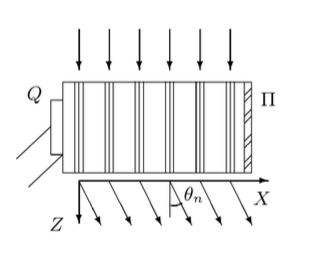
\includegraphics[scale=1.5]{1.png}
	\caption{Дифракция световых волн на акустической решетке}
	\label{diff}
\end{figure}	
	
	
	
При небольших амплитудах звуковой волны показатель преломления жидкости n меняется по закону:
\begin{equation}
	n = n_0 (1 + a \cos K x)
\end{equation}
	
где $K$ - это волновое число для УЗ-волны ($k=\frac{2\phi}{\Lambda}$), $\Lambda$ - длина УЗ-волны, $a$ - глубина модуляции показателя преломления, определяемая интенсивностью ультразвуковой волны ($a<<1$).

Пусть фаза световых колебаний $ \phi $ на передней поверхности жидкости (координата L по оси Z, т.е. толщина водного слоя) равна 0. Тогда на задней поверхности (координата Z=0) фаза равна:

\begin{equation}
	\phi  = k n L = \phi_0 (1 + a \cos K x)
\end{equation}
	
где $ k = 2 \pi / \lambda $ --- волновое число для света, $\lambda $ - длина световой волны, $ L $ --- толщина жидкости в кювете, $\phi_0=kn_0L$.


Фронт прошедшей через кюветы световой волны определяется $z=\dfrac{\phi}{k}$. Угол $\theta(x)$ поворота волнового фронта зависит от координаты $x$:

\begin{equation}
	\theta(x)=\dfrac{dz}{dx}=\dfrac{1}{k}\cdot\dfrac{\phi}{dx}=-\dfrac{K}{k}\phi_0a\sin(Kx)=-Kn_0LaKx
\end{equation}
Учитывая критерий, по которому можно пренебречь искривлением световых лучей $|\theta(x)_{max}L|<<\Lambda$ Получим:

\begin{equation}
	a<<\left(\dfrac{\Lambda}{L}\right)^2
\end{equation}

Таким образом, чисто фазовая акустическая решетка реализуется на достаточно слабой УЗ-волне. При повышении мощности ультразвука акустическая волна начинает работать как сложная амплитудная решетка.

После прохождения через кювету световое поле есть совокупность плоских волн, распространяющихся под углами $ \theta $, соответствующими максимумам в дифракции Фраунгофера:
\begin{equation}	
	\Lambda \sin \theta_m = m \lambda
\end{equation}		
Этот эффект проиллюстрирован на рисунке \ref{diff}.
Зная положение дифракционных максимумов, по формуле (1) легко определить длину ультразвуковой волны, учитывая малость $ \theta $: $ \sin \theta \approx \theta \approx l_m /F  $, где $ l_m $ --- измеренное экспериментально линейное расстояние между m-ым и нулевым максимуми, $ F $ --- фокусное расстояние линзы (объектив $O_2$). Тогда получим:
		
\begin{equation}
	\Lambda = m \lambda F/ l_m 
\end{equation}
Скорость ультразвуковых волн в жидкости, где $ \nu $ --- частота колебаний излучателя:
		
\begin{equation}
	v = \Lambda \nu 
\end{equation}
			
\newpage

\section{Экспериментальная установка}

\begin{figure}[H]
	\centering
	\includegraphics[scale=1.2]{ust.png}
	\caption{Схема наблюдения дифракции установки}
	\label{ust1}
\end{figure}

Источник света Л (рис. \ref{ust1}) с помощью конденсора К проецируется на входную (коллиматорную) щель S. Щель ориентирована вертикально и прикрыта красным светофильтром Ф. Коллиматорный объектив О₁ посылает параллельный пучок на кювету с водой С. Излучатель Q, погруженный в воду, создает УЗ-волну. При определенных положениях излучателя волна становится стоячей. 
Параллельный пучок света, дифрагируя на стоячей звуковой волне, образует дифракционную картину в фокальной плоскости F камерного объектива O₂. Картина наблюдается микроскопом М.

\begin{figure}[H]
	\centering
	\includegraphics[scale=1.2]{ust2.png}
	\caption{Схема наблюдения акустической решётки методом тёмного поля}
	\label{ust2}
\end{figure}

В настоящей работе используется метод тёмного поля для получения видимого изображения решётки, основанный на устранении центрального дифракционного максимума с помощью специального экрана. Результирующее колебание на векторной диаграмме представляется при этом суммой только двух векторов $E_1$ и $E_{-1}$. 

\begin{figure}[H]
	\centering
	\includegraphics[scale=1.2]{vecdig.png}
	\caption{Векторная диаграмма амлитудной решетки}
	\label{vecdig}
\end{figure}

Как следует из диаграммы выше, амплитуда результирующего колебания при этом максимальна при углах поворота векторов $\gamma_1=\gamma_{-1}=0,\phi$ и равна нулю при углах $\gamma_1=\gamma_{-1}=\phi/2, 3\phi/2$. В поле зрения микроскопа наблюдаются чередующиеся светлые и тёмные полосы, причём расстояние между тёмными полосами соответствует смещению в плоскости кюветы на $\Lambda/2$. Таким образом, наблюдается для метода тёмного поля удвоение числа деталей рассматриваемой структуры.
Этот опыт можно проводить только со стоячими волнами, т.к. в случае бегущей волны визуальное наблюдение оказывается невозможным: глаз не успевает следить быстро за перемещающейся волной.

\newpage

\section{Ход работы}
Параметры установки: фокусное расстояние объектива $  O_2  $ $ F = 30 $ см, одно деление винта микроскопа составляет 4 мкм, погрешность измерений примем равной  $ \sigma = $ 2 деления, или 8 мкм.

Исследуем изменения дифракционной картины на зеленом свете. При увеличении частоты УЗ-генератора и приближении к 1,115 МГц проявляется дифракционная решетка: расстояние между максимумами растет.

\begin{enumerate}
\item Измерим положения $ x_m $ дифракционных максимумов с помощью микроскопического винта для четырех частот. Результаты измерений занесены в таблицы 1-4 ниже. На основе каждой таблицы построены графики зависимости $ x_m (m) $, они изображены на рисунке ниже. Коэффициенты углов наклонов прямых для всех зависимостей сведены в таблицу 4.

\newline

\begin{figure}[H]
	\centering
	\includegraphics[scale=0.8]{2pic.jpg}
	\caption{Дифракционная картинка на частоте $\nu=1,115 Мгц$}
	\label{5diff}
\end{figure}	

\begin{table}[!ht]
	\centering
	\begin{tabular}{|c|c|c|c|c|c|}
		\hline
		$m$ &-2&-1&0&1&2\\
		\hline
		$x_m, \ мкм$ &1980&1840& 1720&1580&1440\\
		\hline
	\end{tabular}
	\caption{Измерение координаты m-ого максимума $x_m$ дифракционной картины при частоте генератора $\nu=1,115 Мгц$}
\end{table}

\newline

\begin{figure}[H]
	\centering
	\includegraphics[scale=0.8]{1pic.jpg}
	\caption{Дифракционная картинка на частоте $\nu=1,477 Мгц$}
	\label{3diff}
\end{figure}	

\begin{table}[!ht]
	\centering
	\begin{tabular}{|c|c|c|c|}
		\hline
		$m$ &-1&0&1\\
		\hline
		$x_m, \ мкм$ &1900&1720& 1540\\
		\hline

	\end{tabular}
	\caption{Измерение координаты m-ого максимума $x_m$ дифракционной картины при частоте генератора} $\nu=1,477 Мгц$
\end{table}

\newline

\begin{figure}[H]
	\centering
	\includegraphics[scale=0.5]{3pic.jpg}
	\caption{Дифракционная картинка на частоте $\nu=2,106 Мгц$}
	\label{3diff2}
\end{figure}

\begin{table}[!ht]
	\centering
	\begin{tabular}{|c|c|c|c|}
		\hline
		$m$ &-1&0&1\\
		\hline
		$x_m, \ мкм$ &1980&1720& 1460\\
		\hline
	\end{tabular}
	\caption{Измерение координаты m-ого максимума $x_m$ дифракционной картины при частоте генератора $\nu=2,106 Мгц$}
\end{table}

\item Построим на одной координатной плоскости графики X=X(m) для каждой из частот. 

\begin{figure}[H]
	\centering
	\includegraphics[scale=0.65]{Xm(m).png}
	\caption{Зависимость координаты максимума от его номера}
	\label{g1}
\end{figure}

\item Для каждой частоты генератора рассчитаем длину УЗ-волны. 

\begin{equation}
	\Lambda=\dfrac{F\lambda}{\tan \alpha},
\end{equation}
где $\alpha$ - угол наклона прямых ($l_m/m=\Delta x_m/\Delta m = \tan \alpha$).

И скорость звука:
\begin{equation}
	\vartheta=\nu\Lambda
\end{equation}

\begin{table}[!ht]
	\centering
	\begin{tabular}{|c|c|c|c|c|c|c|}
		\hline
		$\nu, МГц$ & $\tan \alpha$, мкм & $\sigma_{\tan \alpha}$, мкм & $\Lambda$, м & $\sigma_{\Lambda}$, м & $v$, м/с & $\sigma_{v}$, м/с \\ \hline
		1,115 & 134 & 10 & 0,0014 & 0,0001 & 1510 & 113   \\ \hline
		1,477 & 180 & 10 & 0,00101 & 0,00006 & 1489 & 83   \\ \hline
		2,106 & 260 & 10 & 0,00071 & 0,00003 & 1470 & 57   \\ \hline
	\end{tabular}
	\caption{Результаты расчетов длины УЗ волны и скорости звука}
\end{table}

Таким образом, средняя скорость звука:
\[ <\vartheta>=(1490 \pm 113) м/с\]
Скорость звука в воде при комнатной температуре составляет $\vartheta_{theor}=1480 м/с$. Следовательно, полученный экспериментальный результат сходится с табличным в пределах погрешности. 
\end{enumerate}

\section{Определение скорости ультразвука методом темного поля}

Для наблюдения акустической решетки используется метод темного поля, который заключается в устранении центрального дифракционного максимума с помощью непрозрачного экрана. Схема установки показана на рисунке \ref{ust2}.

\begin{enumerate}
	\item Приставим к задней стенке (для светового луча) кюветы стеклянную пластинку с миллиметровыми делениями; сфокусируем микроскоп на изображение пластинки.
	Сторона квадрата сетки: 1 мм. Координаты левого и правого краёв квадрата по шкале микроскопа соответствуют 63 и 84 делениям. Таким образом, цена деления шкалы микроскопа:
	\[ \delta=0,048 мм \]
	
	\item Без применения метода темного поля звуковая решетка не наблюдается. Закроем нулевой максимум горизонтальной нитью. Таким образом, осевая составляющая фазово-модулированной волны поглощается, а боковые остаются без изменения. Получившееся поле: 
	
	\begin{equation}\label{}
		f(x) = \dfrac{im}{2} e^{i\Omega x} +  \dfrac{im}{2} e^{-i\Omega x} = im \cos \Omega x I(x) = m^2 \cos ^2 \Omega x = m^2 \dfrac{1 + \cos ^2 2 \Omega x}{2}
	\end{equation}
	
	Формулы для расчета длины волны ультразвука $ \Lambda $ и скорости распространения $ v $ в воде:
	\begin{equation}\label{}
		\Lambda  = mF\lambda/l_m,  \qquad v = \nu\Lambda
	\end{equation}

	\item После закрытия проволокой центрального максимума определяем координаты первой $x_1$ и последней $x_2$ хорошо видимых полос и количество светлых промежутков между ними n.
	
	Картины наблюдения получились только при частотах 
	\[\nu_1 = 0,819\ МГц \ и \ \nu_2 = 1,052 \ МГц,\] 
	с помощью этих данных можно определить скорость звука и длину волны. 
	
	\begin{table}[!ht]
		\centering
		\begin{tabular}{|c|c|c|c|c|c|}
			\hline
			 $\nu$, МГц & $x_1$, мм & $\sigma_{x_1}$, мм & $x_2$, мм & $\sigma_{x_2}$, мм & n  \\ \hline
			 1,052 & 0,029 & 0,05 & 1,651 & 0,05 & 10  \\ \hline
			0,691 & 0,038 & 0,05 & 1,699 & 0,05 & 13  \\ \hline
		\end{tabular}
		\caption{Результаты измерений координат крайней левой и крайней правой темных полос и число светлых между ними}
	\end{table}
	
	\begin{table}[H]
		\centering
		\begin{tabular}{|c|c|c|c|c|c|c|}
			\hline
			$\nu$, МГц & $l_m$, мм & $\sigma_{l_m}$, мм & $\Lambda$, м & $\sigma_{\Lambda}$, м & $V$, м/с & $\sigma_{v}$, м/с  \\ \hline
			1,052 & 0,16 & 0,07 & 0,0011 & 0,0005 & 1177 & 513  \\ \hline
			0,819 & 0,13 & 0,07 & 0,0014 & 0,0008 & 1163 & 644  \\ \hline
		\end{tabular}
		\caption{Расчеты УЗ-волны}
	\end{table}
	
	Таким образом, средняя скорость звука:
	\[ <\vartheta>=(1170 \pm 643) м/с\]
	 Следовательно, полученный экспериментальный результат сходится с табличным в пределах погрешности. 

\end{enumerate} 
	
\section*{Вывод}
В ходе работы мы наблюдали дифракционную картину после прохождения света через фазовую дифракционную решетку, образованную засчет разных коэффициентов преломления воды, получаемые стоячей УЗ-волной. Рассчитали скорость этой УЗ волны двумя способами: непосредственным наблюдением дифракционной картины и методом темного поля. В обоих случаях результаты сошлись с теоретическим в пределах погрешности. 

\end{document}